% =====================================================
% Problem 4: General Information Retrieval (including Q/A)
% =====================================================

\section{Problem 4: General Information Retrieval (including Q/A)}

\subsection{Problem Description}

This problem introduces classical keyword-based retrieval, semantic search using embeddings, and Retrieval-Augmented Generation (RAG) using a single Arabic book in plain text format as the reference source.

\subsection{Dataset: The Arabic E-Book Corpus.}
The Arabic E-Book Corpus is a freely available collection of 1,745 books (81.5 million words) published by the Hindawi foundation between 2008 and 2024. The books span various genres, including non-fiction, novels, children's literature, poetry, and plays. The corpus is provided in two versions: HTML and unformatted plain text; the latter is used here.

% ------------------------------------------------------------------
\subsection{Book Description}
% ------------------------------------------------------------------

\noindent\textbf{Title \& Source:}
\textarabic{فلسفة الغزالي} (\emph{Al-Ghazali's Philosophy}) by \textarabic{عباس محمود العقاد} (Abbas Mahmoud Al-Aqqad), sourced from the Hindawi Arabic E-Book Corpus (public domain).

\medskip
The book explores the intellectual and philosophical legacy of Imam Abu Hamid Al-Ghazali, one of the most influential thinkers in Islamic history. Known for his strong criticism of the philosophers of his time, Al-Ghazali believed that the spread of certain philosophical ideas had led to religious doubt and moral decline. To challenge these ideas effectively, he deeply studied philosophy himself, producing landmark works such as \emph{Maqasid Al-Falasifa} and \emph{Tahafut Al-Falasifa}.

\medskip
In this concise yet insightful book, Al-Aqqad examines how Al-Ghazali's critiques were not merely attacks on philosophy, but sophisticated philosophical arguments in their own right. He reveals how Al-Ghazali developed a unique intellectual approach that combined logic, theology, and critical analysis --- ultimately shaping a distinct philosophy of thought that continues to influence readers and scholars today.

\medskip
\noindent This topic is uncommon enough that retrieval meaningfully outperforms LLM-only answers, making it well-suited for evaluating RAG benefits.

% ------------------------------------------------------------------
\subsection{Book Preparation for Search}
% ------------------------------------------------------------------

\subsubsection{Text Cleaning and Normalization}

The raw Arabic text is preprocessed in three steps:

\begin{enumerate}
  \item \textbf{Remove diacritics (tashkeel):} Unicode diacritic marks in the range \texttt{U+064B}--\texttt{U+065F} and related code points are stripped using a regular expression.

  \item \textbf{Normalize Arabic letters:} Common orthographic variants are unified to reduce vocabulary fragmentation:
\begin{itemize}
  \item Normalize \textarabic{أ، إ، آ} to \textarabic{ا}.
  \item Normalize \textarabic{ة} to \textarabic{ه}.
  \item Normalize \textarabic{ى} to \textarabic{ي}.
\end{itemize}

  \item \textbf{Remove extra whitespace:} Consecutive whitespace characters are collapsed to a single space and leading/trailing spaces are stripped.
\end{enumerate}

\subsubsection{Splitting into Short Paragraphs}

\begin{enumerate}
  \item \textbf{Sentence segmentation:} The text is split on Arabic sentence-ending markers: full stop, question mark (\textarabic{؟}), exclamation mark, and the \texttt{•••} paragraph separator that appears in this text.

  \item \textbf{Overlapping chunk creation:} Sentences are grouped into chunks of \textbf{2--4 sentences} using a sliding window with a one-sentence overlap (step size = 2). Each chunk is stored as a dictionary containing the chunk text, sentence indices, number of sentences, and character count. The book yielded \textbf{41 chunks} in total.
\end{enumerate}

\subsubsection{Generating Embeddings}

\noindent\textbf{Model:} \texttt{sentence-transformers/paraphrase-multilingual-MiniLM-L12-v2}

\medskip
This sentence-transformer maps sentences and paragraphs to a \textbf{384-dimensional} dense vector space. It supports over 50 languages including Arabic and is efficient enough for CPU inference.

\medskip
Vectors are \textbf{L2-normalized} before indexing so that the inner product between any two vectors equals their cosine similarity. This avoids a costly division at query time:

\begin{align}
  \cos(\theta) &= \frac{\mathbf{A} \cdot \mathbf{B}}{\|\mathbf{A}\|_2 \|\mathbf{B}\|_2}
  \qquad \text{(cosine similarity)} \\[6pt]
  \hat{\mathbf{A}} &= \frac{\mathbf{A}}{\|\mathbf{A}\|_2}
  \qquad \text{(L2 normalization)} \\[6pt]
  \hat{\mathbf{A}} \cdot \hat{\mathbf{B}} &= \frac{\mathbf{A} \cdot \mathbf{B}}{\|\mathbf{A}\|_2\,\|\mathbf{B}\|_2} = \cos(\theta)
\end{align}

\subsubsection{Vector Indexing with FAISS}

A \textbf{FAISS \texttt{IndexFlatIP}} (flat inner-product) index is built over the 41 normalized chunk embeddings. Because the vectors are L2-normalized, inner-product search is equivalent to cosine-similarity search while remaining computationally efficient. The index, chunk metadata, and raw embeddings are all persisted to disk for reuse.

\medskip
\noindent FAISS (Facebook AI Similarity Search) provides efficient algorithms for searching and clustering high-dimensional vectors, making it the standard choice for embedding-based retrieval systems.

% ------------------------------------------------------------------
\subsection{Retrieval System}
% ------------------------------------------------------------------

The system accepts an Arabic query and returns the top-5 results from three retrieval methods simultaneously.

\subsubsection{Arabic Tokenizer}

Before classical retrieval, text is tokenized by:
\begin{enumerate}
  \item Applying the same normalization as in preprocessing (diacritics, letter variants).
  \item Extracting tokens matching Arabic Unicode characters (\texttt{U+0600}--\texttt{U+06FF}).
  \item Removing a curated list of \textbf{Arabic stop words} (e.g., \textarabic{في، هذا، حتى، من، إلى}) that carry minimal semantic meaning and would otherwise inflate matching scores for common terms.
\end{enumerate}

\subsubsection{Classical Search --- TF-IDF}

TF-IDF (Term Frequency -- Inverse Document Frequency) ranks a document by how frequently a query term appears in it (TF), discounted by how common that term is across the entire corpus (IDF):

\begin{equation}
  \text{score}(t, d) = \underbrace{\frac{f_{t,d}}{|d|}}_{\text{TF}} \times \underbrace{\log\!\left(\frac{N+1}{\text{df}(t)+1}\right)+1}_{\text{IDF (smoothed)}}
\end{equation}

Document vectors are L2-normalized and ranked against the query vector by cosine similarity.

\subsubsection{Classical Search --- BM25}

BM25 (Best Matching 25) extends TF-IDF by incorporating \emph{term-frequency saturation} (high TF yields diminishing returns) and \emph{document-length normalization}:

\begin{equation}
  \text{score}(q, d) = \sum_{t \in q} \text{IDF}(t) \cdot \frac{f_{t,d}\,(k_1+1)}{f_{t,d} + k_1\!\left(1 - b + b\,\dfrac{|d|}{\text{avgdl}}\right)}
\end{equation}

with hyperparameters $k_1 = 1.5$ and $b = 0.75$.

\subsubsection{Semantic Search}

The query is encoded by the same \texttt{paraphrase-multilingual-MiniLM-L12-v2} model, L2-normalized, and used to query the FAISS index via inner-product search. This method retrieves semantically related passages even when the query uses different vocabulary from the document.

% ------------------------------------------------------------------
\subsection{RAG System}
% ------------------------------------------------------------------

\subsubsection{Language Model Selection}

\paragraph{First attempt --- \texttt{Qwen/Qwen2.5-1.5B-Instruct}.}
Qwen2.5-1.5B-Instruct is a lightweight 1.54-billion parameter causal language model from Alibaba Cloud, designed for instruction following with multilingual capabilities and a 32,768-token context window (Apache 2.0 license). However, due to its strong pretraining bias toward Chinese data and its small size --- which limits cross-lingual adherence --- the model defaulted to Chinese responses even for Arabic prompts, as shown in Figure~\ref{fig:qwen_chinese}.

\begin{figure}[H]
  \centering
  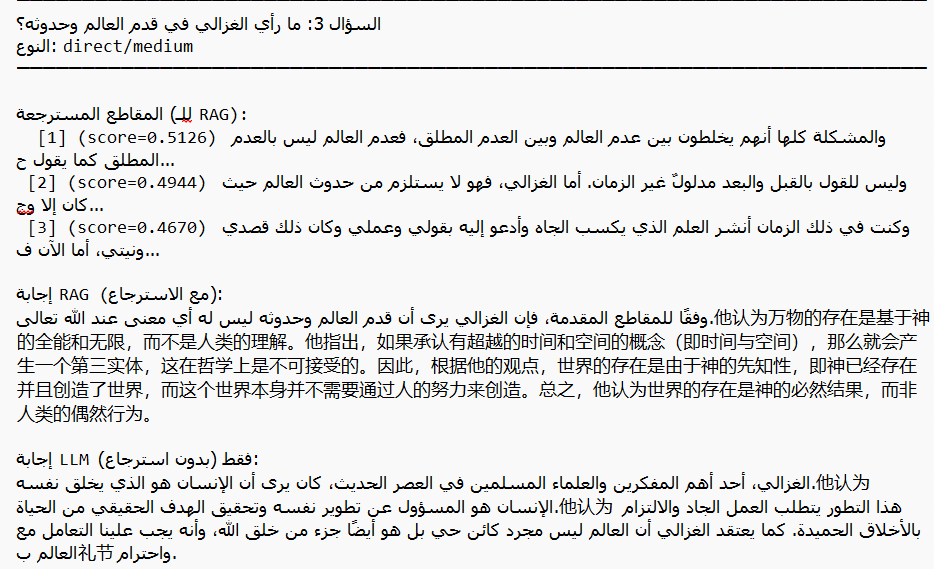
\includegraphics[width=0.65\textwidth]{figures/Hallucination.png}
  \caption{Qwen2.5-1.5B-Instruct defaulting to Chinese when prompted in Arabic.}
  \label{fig:qwen_chinese}
\end{figure}

\paragraph{Final model --- \texttt{silma-ai/SILMA-Kashif-2B-Instruct-v1.0}.}
SILMA Kashif 2B Instruct v1.0 is the premier release of the SILMA Kashif model family, developed by SILMA AI. With 2 billion parameters, it is \textbf{specifically designed for RAG tasks} in Arabic and English, excelling at answering questions grounded in retrieved context. It also supports entity extraction as a secondary capability.

\subsubsection{Prompts}

\noindent\textbf{System prompt (both modes):}
\begin{tcolorbox}[colback=pygray, colframe=black!30, boxrule=0.4pt, arc=2pt, left=6pt, right=6pt, top=4pt, bottom=4pt, fontupper=\ttfamily\footnotesize]
\textarabic{أنت مساعد ذكي متخصص في الفلسفة الإسلامية. أجب على الأسئلة بدقة وباللغة العربية.}
\end{tcolorbox}

\noindent\textbf{RAG prompt template} (retrieved context injected):
\begin{tcolorbox}[colback=pygray, colframe=black!30, boxrule=0.4pt, arc=2pt, left=6pt, right=6pt, top=4pt, bottom=4pt, fontupper=\ttfamily\footnotesize]
\textarabic{أنت مساعد متخصص في الفلسفة الإسلامية. استخدم المقاطع التالية من كتاب "فلسفة الغزالي" للإجابة على السؤال.}\\
\\
\textarabic{المقاطع المسترجعة:}\\
\{context\}\\
\\
\textarabic{السؤال:} \{question\}\\
\\
\textarabic{الإجابة (بالعربية):}
\end{tcolorbox}

\noindent\textbf{LLM-only prompt template} (no retrieval):
\begin{tcolorbox}[colback=pygray, colframe=black!30, boxrule=0.4pt, arc=2pt, left=6pt, right=6pt, top=4pt, bottom=4pt, fontupper=\ttfamily\footnotesize]
\textarabic{أنت مساعد متخصص في الفلسفة الإسلامية. أجب على السؤال التالي من معرفتك العامة.}\\
\\
\textarabic{السؤال:} \{question\}\\
\\
\textarabic{الإجابة (بالعربية):}
\end{tcolorbox}

\subsubsection{RAG Pipeline}

For each question the system executes the following steps:

\begin{enumerate}
  \item \textbf{Semantic retrieval:} The top-3 most relevant chunks are retrieved from the FAISS index using the query embedding.
  \item \textbf{Context assembly:} The retrieved chunks are concatenated with numbered labels and inserted into the RAG prompt template.
  \item \textbf{RAG generation:} The populated prompt is passed to SILMA Kashif, producing a grounded Arabic answer.
  \item \textbf{LLM-only generation:} The same question is passed to the model using the LLM-only template (no retrieved context), producing a baseline answer from parametric knowledge alone.
  \item \textbf{Display:} Both answers are displayed side by side for comparison.
\end{enumerate}

% ------------------------------------------------------------------
\subsection{Interface}
% ------------------------------------------------------------------

A desktop GUI was built with \textbf{PySimpleGUI}. It has three tabs:

\begin{itemize}
  \item \textbf{Retrieval tab:} Accepts an Arabic query and displays top-5 results from TF-IDF, BM25, and Semantic search in three parallel columns (Figure~\ref{fig:interface_retrieval}).
  \item \textbf{Question answering tab:} Accepts an Arabic question, shows the retrieved chunks from the book, then displays the RAG answer and the LLM-only answer side by side (Figure~\ref{fig:interface_qa}).
  \item \textbf{System info tab:} Displays book metadata, model names, and FAISS index details (Figure~\ref{fig:interface_info}).
\end{itemize}

\begin{figure}[H]
  \centering
  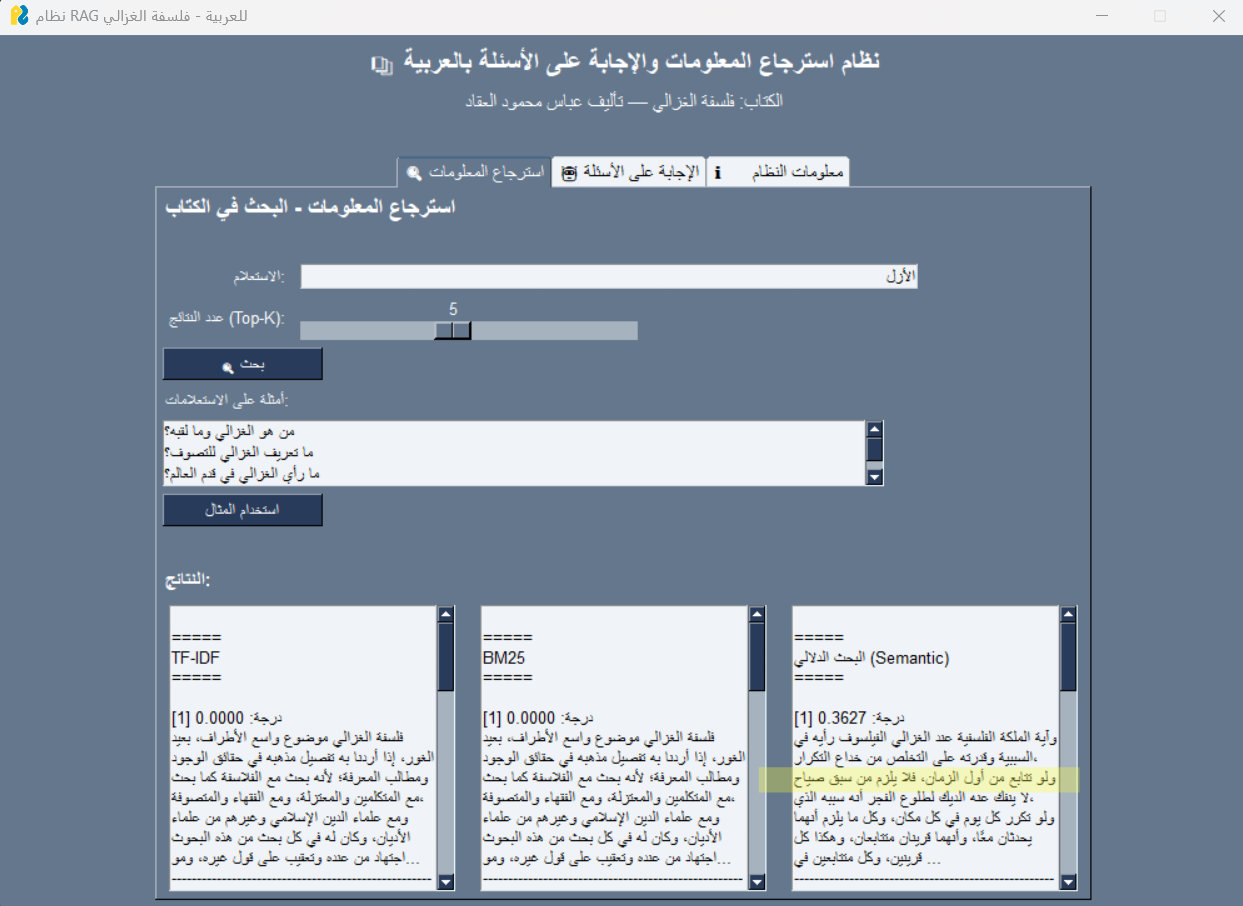
\includegraphics[width=0.7\textwidth]{figures/Retrieval.png}
  \caption{Interface --- Retrieval tab: TF-IDF, BM25, and Semantic results displayed in parallel columns. Note how semantic search surfaces a relevant passage about \textarabic{أول الزمان} (start oftime) in response to a query containing \textarabic{الأزل} (eternity) --- a synonym not present in the text.}
  \label{fig:interface_retrieval}
\end{figure}

\begin{figure}[H]
  \centering
  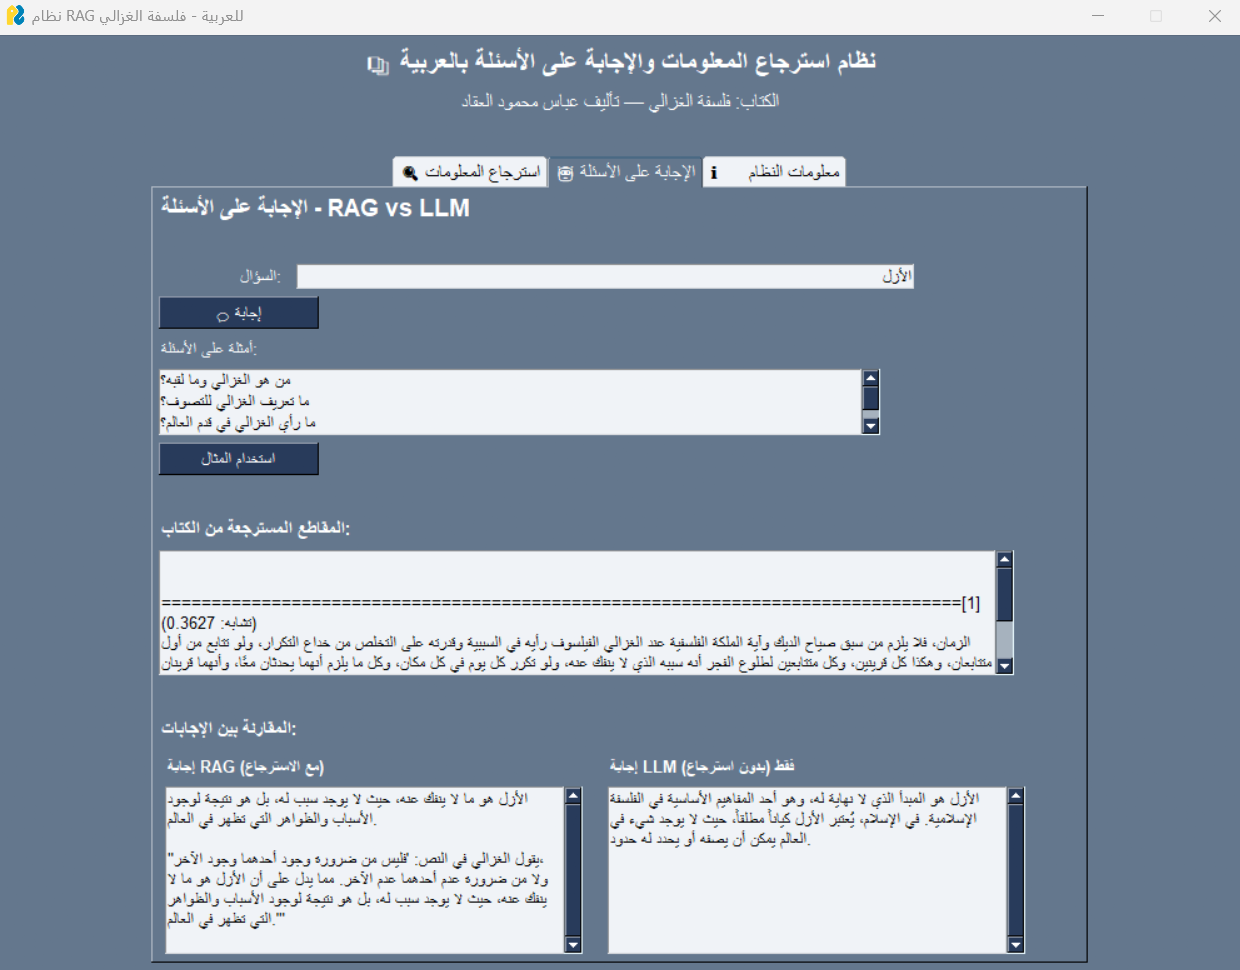
\includegraphics[width=0.7\textwidth]{figures/Question Answering.png}
  \caption{Interface --- Question answering tab: retrieved context (top), RAG answer (left), and LLM-only answer (right).}
  \label{fig:interface_qa}
\end{figure}

\begin{figure}[H]
  \centering
  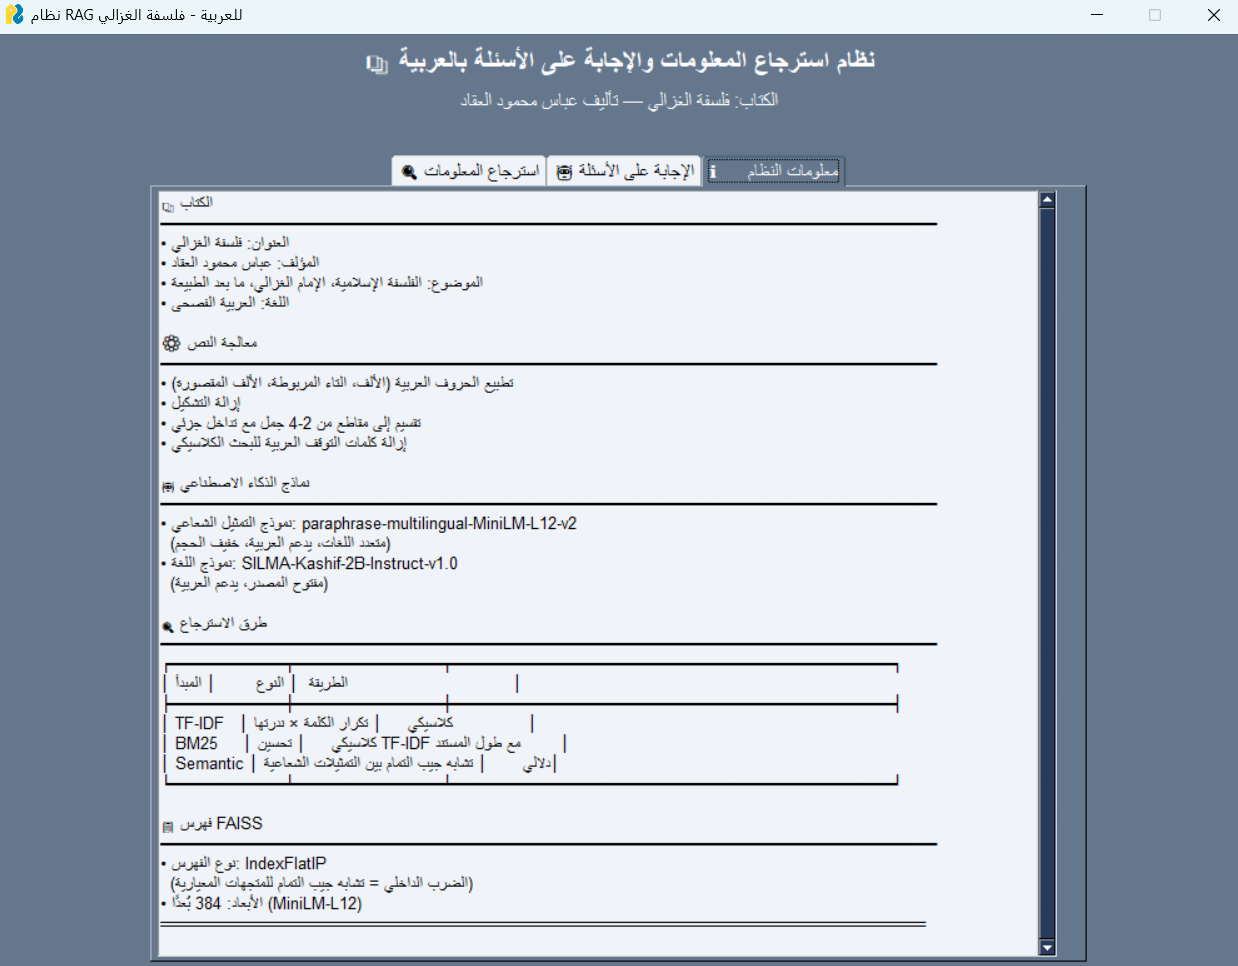
\includegraphics[width=0.7\textwidth]{figures/System Info.png}
  \caption{Interface --- System info tab: book details, model specifications, and FAISS index configuration.}
  \label{fig:interface_info}
\end{figure}

% ------------------------------------------------------------------
\subsection{Experiments and Results}
% ------------------------------------------------------------------

\subsubsection{Evaluation Queries}

Ten Arabic queries were designed to cover a range of difficulty and question types, as shown in Table~\ref{tab:queries}.

\begin{table}[H]
  \centering
  \caption{The 10 evaluation queries with type classification.}
  \label{tab:queries}
  \renewcommand{\arraystretch}{1.35}
  \begin{tabularx}{\textwidth}{c l X}
    \toprule
    \textbf{\#} & \textbf{Type} & \textbf{Query} \\
    \midrule
    1  & Direct / Easy    & \textarabic{من هو الغزالي وما لقبه؟} \\
    2  & Direct / Easy    & \textarabic{ما هو تعريف الغزالي للتصوف؟} \\
    3  & Direct / Medium  & \textarabic{ما رأي الغزالي في قدم العالم وحدوثه؟} \\
    4  & Direct / Medium  & \textarabic{كيف يختلف الغزالي عن الفلاسفة في مسألة الزمان؟} \\
    5  & Direct / Medium  & \textarabic{ما هو موقف الغزالي من السببية وهل ينكرها؟} \\
    6  & Indirect / Medium & \textarabic{لماذا كان الغزالي أقدر من الفلاسفة أنفسهم؟} \\
    7  & Indirect / Medium & \textarabic{ما العلاقة بين التصوف والفلسفة عند الغزالي؟} \\
    8  & Direct / Hard    & \textarabic{كيف فسّر الغزالي مسألة البعث والنفس والجسد؟} \\
    9  & Indirect / Hard  & \textarabic{كيف تُعدّ رياضة الغزالي النفسية خطوة فلسفية وليست دينية فقط؟} \\
    10 & Indirect / Hard  & \textarabic{ما الفرق بين التفكير العلمي التجريبي والتفكير الفلسفي عند الغزالي؟} \\
    \bottomrule
  \end{tabularx}
\end{table}

\subsubsection{Retrieval and RAG Results}

Full result tables --- including top-5 retrieved passages per method for all 10 queries, and RAG vs.\ LLM-only answers for both \texttt{Qwen2.5-1.5B-Instruct} and \texttt{SILMA-Kashif-2B-Instruct-v1.0} --- are saved to:

\begin{itemize}
  \item \texttt{outputs/evaluation\_report.txt} (Qwen model)
  \item \texttt{outputs\_silma/evaluation\_report.txt} (SILMA model)
\end{itemize}

% ------------------------------------------------------------------
\subsection{Comparison and Reflection}
% ------------------------------------------------------------------

\subsubsection{Which Retrieval Method Produced More Relevant Results?}

\begin{itemize}
  \item \textbf{Semantic search} excels for indirect questions, paraphrased queries, and conceptual questions. For example, a query containing \textarabic{الأزل} (eternity) successfully retrieved passages about \textarabic{الزمان} (time) --- a semantically related term that does not appear verbatim in the query.
  \item \textbf{BM25 and TF-IDF} perform well when the query contains exact terms from the text, such as specific Arabic philosophical terminology like \textarabic{السببية} (causality) or \textarabic{البعث} (resurrection).
  \item For Arabic specifically, semantic search overcomes the challenge of \textbf{morphological variants}: the same root word can produce dozens of surface forms, which classical methods treat as distinct tokens.
\end{itemize}

\subsubsection{Did Retrieval Improve LLM-Generated Answers?}

\begin{itemize}
  \item \textbf{Yes, significantly} for book-specific questions. The LLM alone tends to produce generic Islamic philosophy answers drawn from pretraining data.
  \item RAG \textbf{anchors answers} to the specific arguments made by Al-Aqqad about Al-Ghazali, producing more faithful, on-topic responses.
  \item LLM-only answers occasionally \textbf{hallucinate} specific quotes or positions; RAG prevents this by grounding generation in retrieved text from the actual book.
\end{itemize}

\subsubsection{Conclusions on Semantic Retrieval and RAG for Arabic Text}

\begin{itemize}
  \item Multilingual sentence-transformer models handle Arabic well despite the language's complex morphology, producing high-quality embeddings that capture semantic similarity across paraphrased queries.
  \item FAISS provides efficient similarity search even on CPU-only hardware, making the pipeline accessible without GPU resources.
  \item RAG effectively bridges the gap between a small LLM's limited parametric knowledge and the specific content of a specialized Arabic text, demonstrating strong value for domain-specific Arabic NLP applications.
\end{itemize}